\documentclass[aspectratio=169, 11pt, invertlogo]{ismll-slides}
% - logo=[all, frametitle, headline, none]
% - logotitlepage=[true, false]
% - invertlogo: where to use white instead of black text (on transparent background)
% - nopdfpagenumbers: disable adding a number for each frame to pdf toc

%%%%%%%%%%%%%%%%
% BEAMER THEME %
%%%%%%%%%%%%%%%%
\usetheme[block=fill, background=light, progressbar=foot, numbering=counter]{metropolis}
%\usetheme{Madrid}
\setbeamertemplate{blocks}[default]
\setbeamercovered{transparent}

%%%%%%%%%%%%%%%%
% BIBLIOGRAPHY %
%%%%%%%%%%%%%%%%
% NOTE: Bibliography should be compiled with biber!
\addbibresource{slides-bibliography.bib}


%%%%%%%%%%%%%%%%%%%%%%%%%%
% TITLE PAGE INFORMATION %
%%%%%%%%%%%%%%%%%%%%%%%%%%

\title{Research Presentation}
\subtitle{Active Learning with V-Learning}
\author{Thorben Werner}
\date{March 31, 2022}
\institute{Information Systems and Machine Learning Lab (ISMLL)\\Institute for Computer Science \\ University of Hildesheim}



\begin{document}

%%%%%%%%%%%%%%%%%%%%%%%%%%%%%%%%%%%%%%%%%%%%%%%%%%%%%%%%%%%%%%%%%%%%%%%%%%%%%%%%%%%%%%%%%%%%%%%%%%%
\maketitle
%%%%%%%%%%%%%%%%%%%%%%%%%%%%%%%%%%%%%%%%%%%%%%%%%%%%%%%%%%%%%%%%%%%%%%%%%%%%%%%%%%%%%%%%%%%%%%%%%%%

\begin{frame}[fragile]{Pool-Based Active Learning}
	\begin{columns}
		\begin{column}{.3\linewidth}
			\begin{align*}
				\mathcal{L} &\in \mathbb{R}^{\lambda \times m} \hspace{3mm}\text{Labeled Set} \\
				\mathcal{U} &\in \mathbb{R}^{\mu \times m} \hspace{3mm}\text{Unlabeled Set} \\
				\phi_\theta &:= \mathbb{R}^{m} \rightarrow \mathbb{R}^{c} \hspace{3mm}\text{Classifier} \\
				\mathcal{K} &\in \mathbb{R}^{k \times m} \hspace{3mm}\text{Unlabeled Sample} \\
				\psi &:= \mathbb{R}^{k \times m} \rightarrow \mathbb{R}^k \hspace{3mm}\text{Active Learning Heuristic} \\
				\pi_\psi &:= argmax \hspace{1mm} \psi(\mathcal{S}) \hspace{3mm}\text{Active Learning Policy}
			\end{align*}
		\end{column}
		\begin{column}{.5\linewidth}
			\begin{figure}
				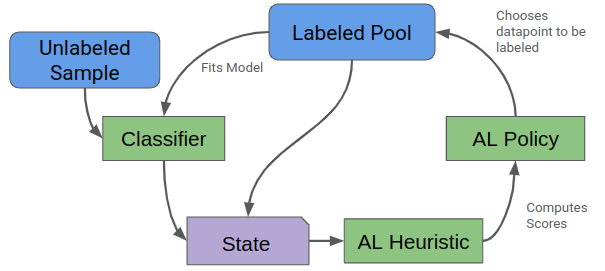
\includegraphics[width=\linewidth]{pics/al_cycle}
				\caption*{Active Learning Cycle}
			\end{figure}
		\end{column}
	\end{columns}
\end{frame}


%%%%%%%%%%%%%%%%%%%%%%%%%%%%%%%%%%%%%%%%%%%%%%%%%%%%%%%%%%%%%%%%%%%%%%%%%%%%%%%%%%%%%%%%%%%%%%%%%%%

\begin{frame}[fragile]{Active Learning with Q-Learning}
	\textbf{State Space:} \\ [2mm]
	\begin{enumerate}
		\item Internal state of the environment: content of labeled pool $\mathcal{L}$, state of the classifier $\theta$, remaining budget, current F1-Score, etc. $\rightarrow \mathbb{R}^{a}$
		\item Information about the unlabeled sample $\mathcal{K}$: Output of the classifier $\phi_\theta(k_t)$, the datapoints themselves, other metrics, etc. $\rightarrow \mathbb{R}^{k \times b}$
	\end{enumerate}
	Results in a flattened state space of $\mathcal{S} \in \mathbb{R}^{a + k \times b}$ \\
	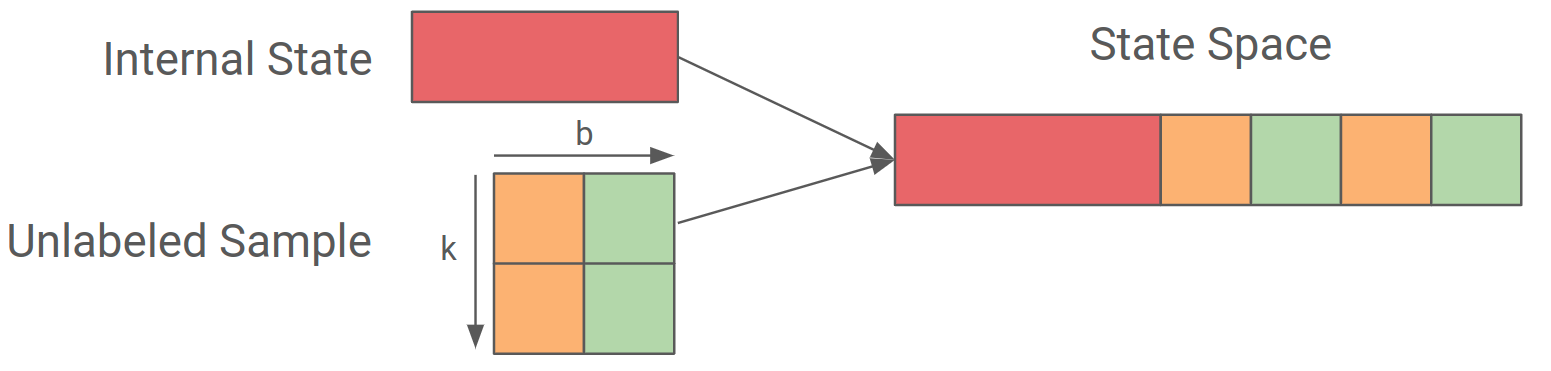
\includegraphics[width=.9\linewidth]{pics/state_space}
\end{frame}


%%%%%%%%%%%%%%%%%%%%%%%%%%%%%%%%%%%%%%%%%%%%%%%%%%%%%%%%%%%%%%%%%%%%%%%%%%%%%%%%%%%%%%%%%%%%%%%%%%%

\begin{frame}[fragile]{Active Learning with Q-Learning}
\begin{columns}
	\begin{column}{.4\linewidth}
		\begin{align*}
		\mathcal{A} &\in [0, \ldots, k] \hspace{3mm}\text{Action Space} \\
		\mathcal{R} &:= \mathcal{S} \times \mathcal{A} \rightarrow \mathbb{R} \hspace{3mm}\text{Reward Function} \\
		\tau &:= \{ \mathcal{S}, \mathcal{A}, \mathcal{S}, \mathcal{R}, \mathbb{R} \} \hspace{3mm}\text{Transition} \\
		\end{align*}
	\end{column}
	\begin{column}{.4\linewidth}
		\textbf{Problems:}
		\begin{itemize}
			\item Fixed Sample size
			\item Expensive Transitions
			\item Same actions in different places
		\end{itemize}
	\end{column}
\end{columns}
\end{frame}


%%%%%%%%%%%%%%%%%%%%%%%%%%%%%%%%%%%%%%%%%%%%%%%%%%%%%%%%%%%%%%%%%%%%%%%%%%%%%%%%%%%%%%%%%%%%%%%%%%%

\begin{frame}[fragile]{Active Learning with Q-Learning}
	\begin{columns}
		\begin{column}{.5\linewidth}
			\textbf{Sample Size} $k=2$ \\ [2mm]
			The same datapoint can appear in multiple places in the input \\[2mm]
			Both output nodes essentially learn the same function since the datapoints are sampled randomly and independently. \\ [2mm]
			A permutation invariant network can fix the problem and create a ranking of actions
		\end{column}
		\begin{column}{.4\linewidth}
			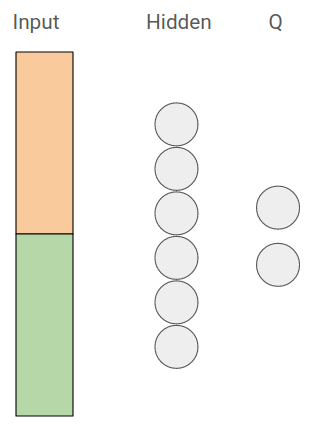
\includegraphics[width=160px]{pics/q}
		\end{column}
	\end{columns}
\end{frame}


%%%%%%%%%%%%%%%%%%%%%%%%%%%%%%%%%%%%%%%%%%%%%%%%%%%%%%%%%%%%%%%%%%%%%%%%%%%%%%%%%%%%%%%%%%%%%%%%%%%

\begin{frame}[fragile]{The Bellman Target}
	\textbf{Q-Learning Target:}
	What is the expected discounted improvement in F1-Score under the current policy when we choose a given datapoint? \\ [2mm]
	The Bellman target does not rank actions, but tries to estimate their independent, global value under the current policy
	\vspace{5mm}
	\begin{columns}
		\begin{column}{.42\linewidth}
			\textbf{Reinforcement Learning} \\ 
			$\mathcal{L}_Q := \hat{\pi}(s_t, a_t) - r_t + \gamma \hspace{1mm} \underset{a}{\operatorname{max}}(\pi(s_{t+1}))$ \\
			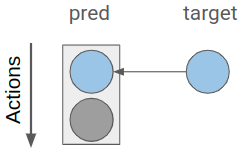
\includegraphics[width=100px]{pics/bellman}
		\end{column}
		\hspace{1mm}
		\begin{column}{.55\linewidth}
			\textbf{Ranking (Triplet Loss)} \\ 
			$\mathcal{L}_{triplet} := max(0, m+d(z_a, z_p) - d(z_a, z_n))$ \\
			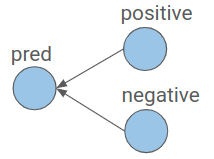
\includegraphics[width=88px]{pics/triplet}
		\end{column}
	\end{columns}
\end{frame}


%%%%%%%%%%%%%%%%%%%%%%%%%%%%%%%%%%%%%%%%%%%%%%%%%%%%%%%%%%%%%%%%%%%%%%%%%%%%%%%%%%%%%%%%%%%%%%%%%%%

\begin{frame}[fragile]{V-Learning vs Q-Learning}
	TODO
\end{frame}

%%%%%%%%%%%%%%%%%%%%%%%%%%%%%%%%%%%%%%%%%%%%%%%%%%%%%%%%%%%%%%%%%%%%%%%%%%%%%%%%%%%%%%%%%%%%%%%%%%%

\begin{frame}[fragile]{Active Learning with V-Learning}
	\begin{columns}
		\begin{column}{.4\linewidth}
			\textbf{Adaptations}
			\begin{itemize}
				\item We use the batch dimension for representing the sample size $k$
				\item No action space needed
				
			\end{itemize}
		\end{column}
		\begin{column}{.4\linewidth}
			\begin{align*}
			\mathcal{S} &\in \mathbb{R}^{\sigma} \hspace{3mm}\text{State Space} \\
			\mathcal{R} &:= \mathcal{S} \rightarrow \mathbb{R} \hspace{3mm}\text{Reward Function} \\
			V_\theta &:= \mathcal{S} \rightarrow \mathbb{R} \hspace{3mm}\text{Agent Network} \\
			\end{align*}
		\end{column}
	\end{columns}
\end{frame}


%%%%%%%%%%%%%%%%%%%%%%%%%%%%%%%%%%%%%%%%%%%%%%%%%%%%%%%%%%%%%%%%%%%%%%%%%%%%%%%%%%%%%%%%%%%%%%%%%%%

\begin{frame}[fragile]{Active Learning with V-Learning}
	Example:
	\begin{align*}
		\text{State is generated} &: s \in \mathbb{R}^{b \times \sigma} \\
		\text{Agents makes prediction} &: v = V_\theta(s) \\
		\text{\textbf{Policy selects a point}} &: a = \underset{b}{\text{argmax }} v_{b} \\
		\text{Action is applied} &: s' = \text{env}(a) \\
		\text{Reward is observed} &: r = \mathcal{R}(s') \\
		\text{Transition is stored} &: \tau = \{ s_{a}, r, \bar s', \text{done} \} \\
		\text{\textbf{with}} &: \bar s' = \frac{1}{b} \sum\limits_{i=0}^b s'_{i}
	\end{align*}
\end{frame}


%%%%%%%%%%%%%%%%%%%%%%%%%%%%%%%%%%%%%%%%%%%%%%%%%%%%%%%%%%%%%%%%%%%%%%%%%%%%%%%%%%%%%%%%%%%%%%%%%%%

\begin{frame}[fragile]{Storing Transitions in Memory}
	Q-Learning:
	\begin{align*}
		O(\tau) &= s \times a \times s' \times r \times \mathbb{R} \\
		O(\tau) &= k^2 \times \sigma^2 + 3
	\end{align*}
	V-Learning:
	\begin{align*}
		O(\tau) &= s_a \times a \times \bar s' \times r \times \mathbb{R} \\
		O(\tau) &= 2 \times \sigma^2 + 3
	\end{align*}
\end{frame}



%%%%%%%%%%%%%%%%%%%%%%%%%%%%%%%%%%%%%%%%%%%%%%%%%%%%%%%%%%%%%%%%%%%%%%%%%%%%%%%%%%%%%%%%%%%%%%%%%%%
\appendix
%%%%%%%%%%%%%%%%%%%%%%%%%%%%%%%%%%%%%%%%%%%%%%%%%%%%%%%%%%%%%%%%%%%%%%%%%%%%%%%%%%%%%%%%%%%%%%%%%%%


%\begin{frame}[fragile]{Backup Slides}
%
%\begin{block}<1->{Did you know?}%
%  Pages after the \verb|\appendix| command do not get counted in the page total.
%\end{block}%
%
%\end{frame}


%%%%%%%%%%%%%%%%%%%%%%%%%%%%%%%%%%%%%%%%%%%%%%%%%%%%%%%%%%%%%%%%%%%%%%%%%%%%%%%%%%%%%%%%%%%%%%%%%%%


\begin{frame}[allowframebreaks]%{References}
%
%\printbibliography%[heading=none]
%
\end{frame}

%%%%%%%%%%%%%%%%%%%%%%%%%%%%%%%%%%%%%%%%%%%%%%%%%%%%%%%%%%%%%%%%%%%%%%%%%%%%%%%%%%%%%%%%%%%%%%%%%%%


\end{document}
